% Chapter 5
\chapter{将非简单多边形标准化}
通常情况下,我们处理的多边形为边界互不相交的简单多边形。对于边界产生了交叉的复杂多边形,需要先进行分割处理,使其变为等价的数个简单多边形。

在判断复杂多边形所覆盖范围时,有着多种可行的定义方法。此处我们采用的定义为:对于一个点,从该点向多边形外无限远处连接任意一条射线,当且仅当该射线与多边形边界相交奇数次时点在多边形内部。

如图\ref*{complex}所示,该复杂多边形由六个顶点组成,所包含的区域用浅蓝色表示。

\begin{figure}[htp]
    \centering
    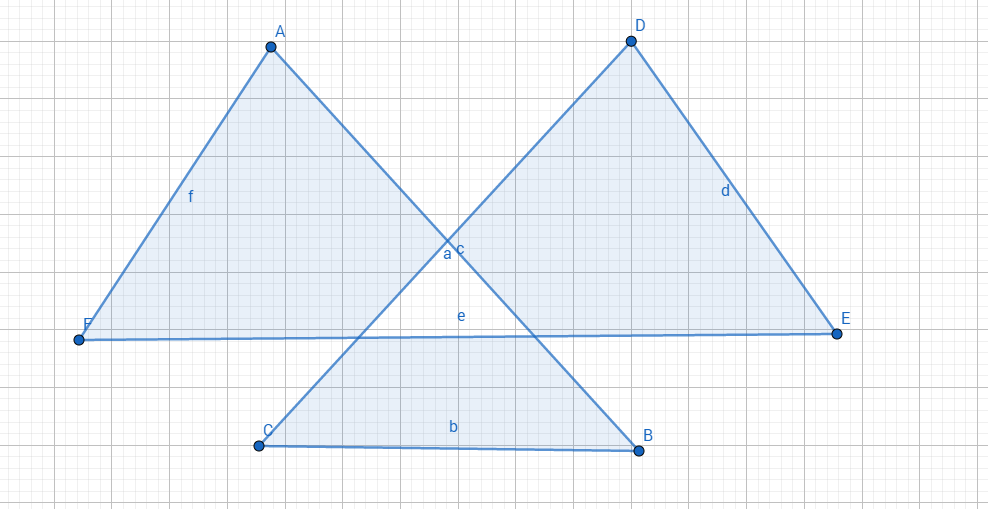
\includegraphics[width=0.5\textwidth]
    {figures/complex.png}
    \caption{复杂多边形的示例}
    \label{complex}
  \end{figure}

由于多边形的边界为一条闭合折线,易知对于每个多边形边界上的顶点,与其连接的边为偶数条。因此,射线的位置对相交次数的奇偶性不产生影响。

明确了划分规则后,我们可以采用逐层分离的方法将原多边形分割为简单多边形的组合。具体方法如下:

\begin{enumerate}
    \item 首先,对于多边形的边界,找出所有未被记录的交叉点,并将对应相交的边分别从交叉点处分割为两部分。
    \item 选择当前点集中x坐标最小的点,作为新多边形的起始点。
    \item 遍历当前点的所有连边,按极角序选择当前点到上一个点连线方向顺时针连接到的第一条边\footnote{对于第一个点从x轴负方向开始},将另一个端点加入当前多边形。
    \item 转到3 直至返回初始点。
    \item 记录当前多边形,并删除当前多边形对应的边和连边数小于2的顶点。
    \item 转到2 直至点集为空。
    \item 对于切割出的每个多边形,计算其内部到多边形外跨越的边数,判断其是否为孔洞。
\end{enumerate}

该算法的本质是记录所有未被顶点标记的交叉点,并重新计算原多边形的边界,判断多边形中每一条边具体所属的多边形边界曲线。

经过以上处理,我们完成了非简单多边形的标准化。自此,我们可以计算出任意多边形的三角剖分。
